\chapter{Intervenções}\label{ape:intervencoes}

No decorrer do minicurso, foram realizadas 12 intervenções por e-mail e pelo mural
de recados para estimular os alunos de ambos os grupos (i.e., os alunos que usaram o Sistema de Recomendação Tradicional
ou a proposta desse trabalho) a acessar o ambiente de aula e se aprofundar nos materiais instrucionais
liberados. Cada uma dessas intervenções e sua respectiva data é apresentada abaixo. As intervenções utilizadas foram adaptadas
de \citeonline{santos2017addie}.

\begin{figure}[htb]
  \caption{\label{fig:intervencao-1}Intervenção 1 (16/04/18)}
  \begin{center}
      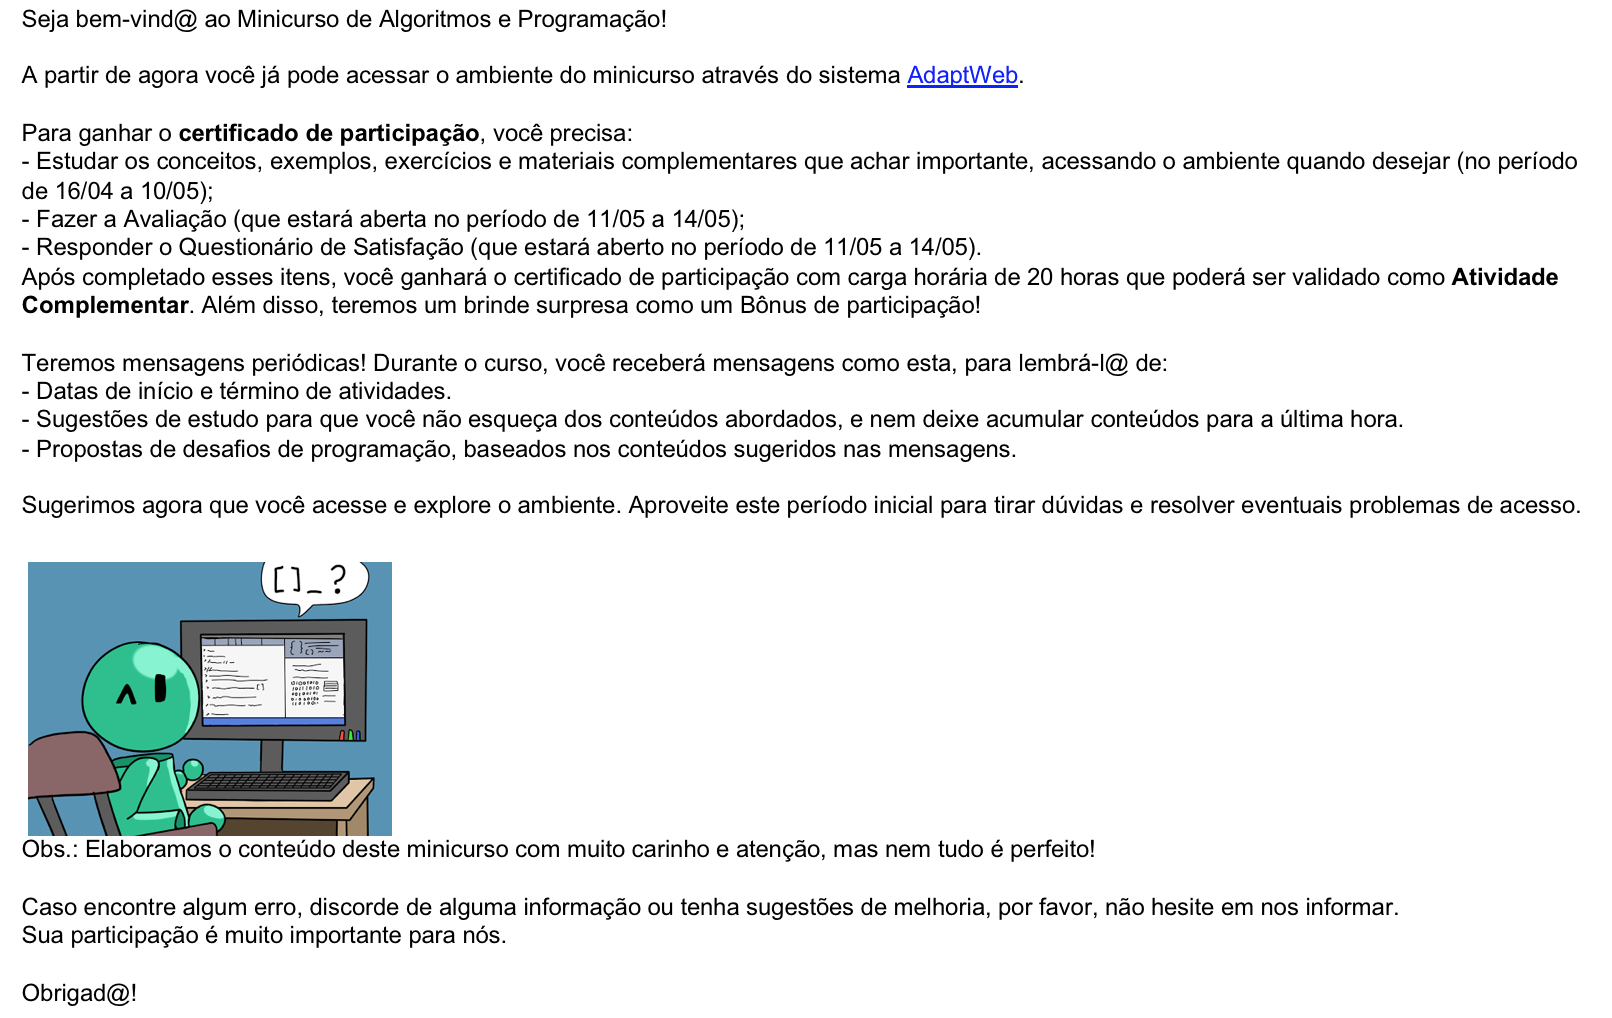
\includegraphics[scale=0.6]{./Figuras/intervencao-1.png}
  \end{center}
  \legend{Fonte: O autor.}
\end{figure}

\begin{figure}[htb]
  \caption{\label{fig:intervencao-2}Intervenção 2 (18/04/18)}
  \begin{center}
      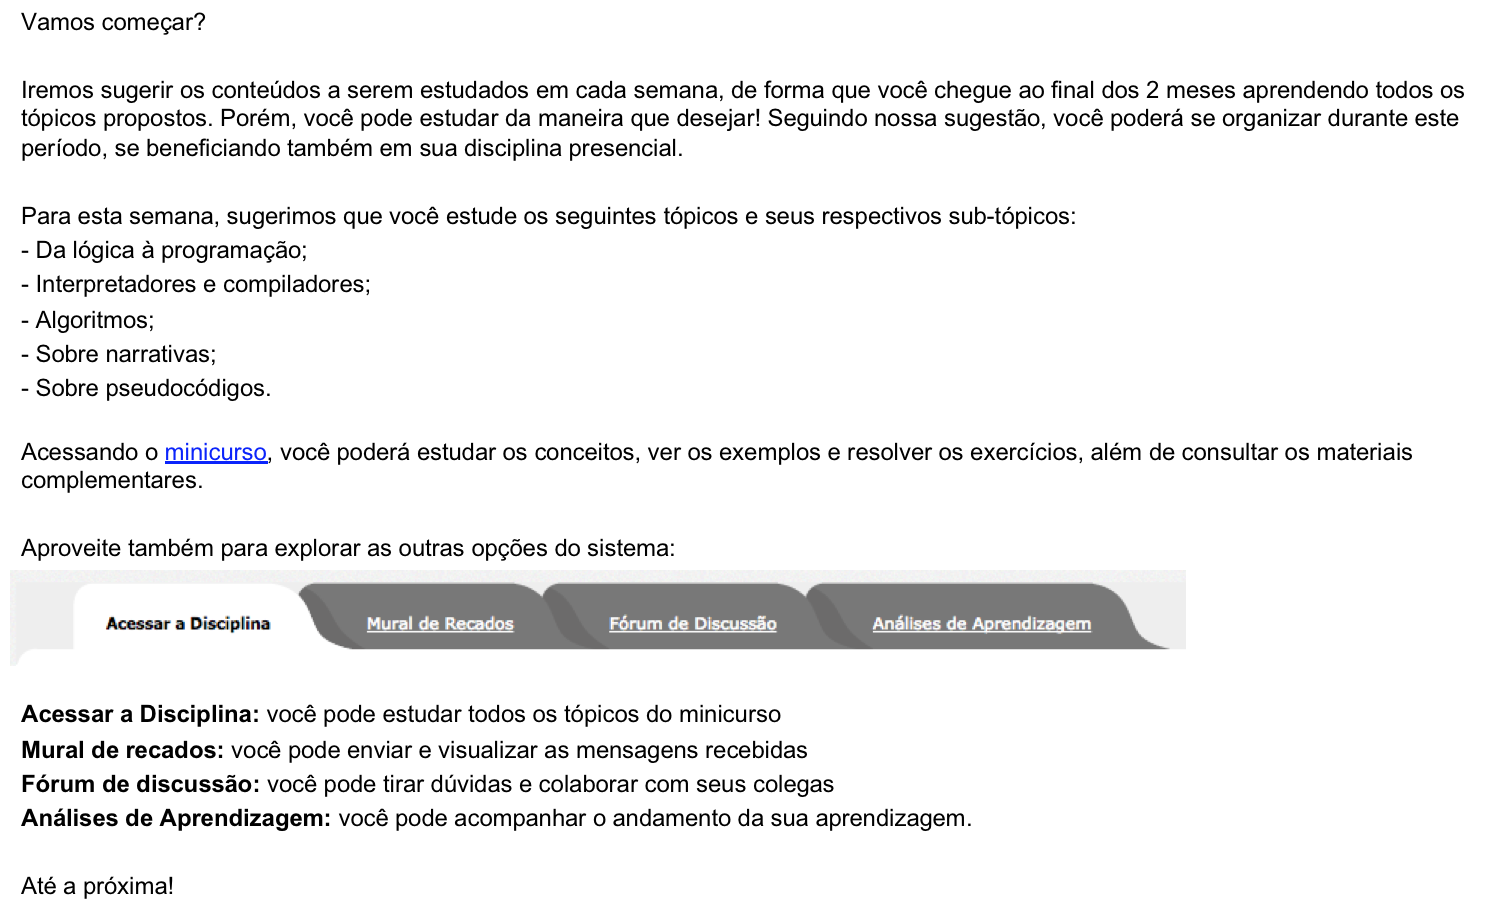
\includegraphics[scale=0.6]{./Figuras/intervencao-2.png}
  \end{center}
  \legend{Fonte: O autor.}
\end{figure}

\begin{figure}[htb]
  \caption{\label{fig:intervencao-3}Intervenção 3 (20/04/18)}
  \begin{center}
      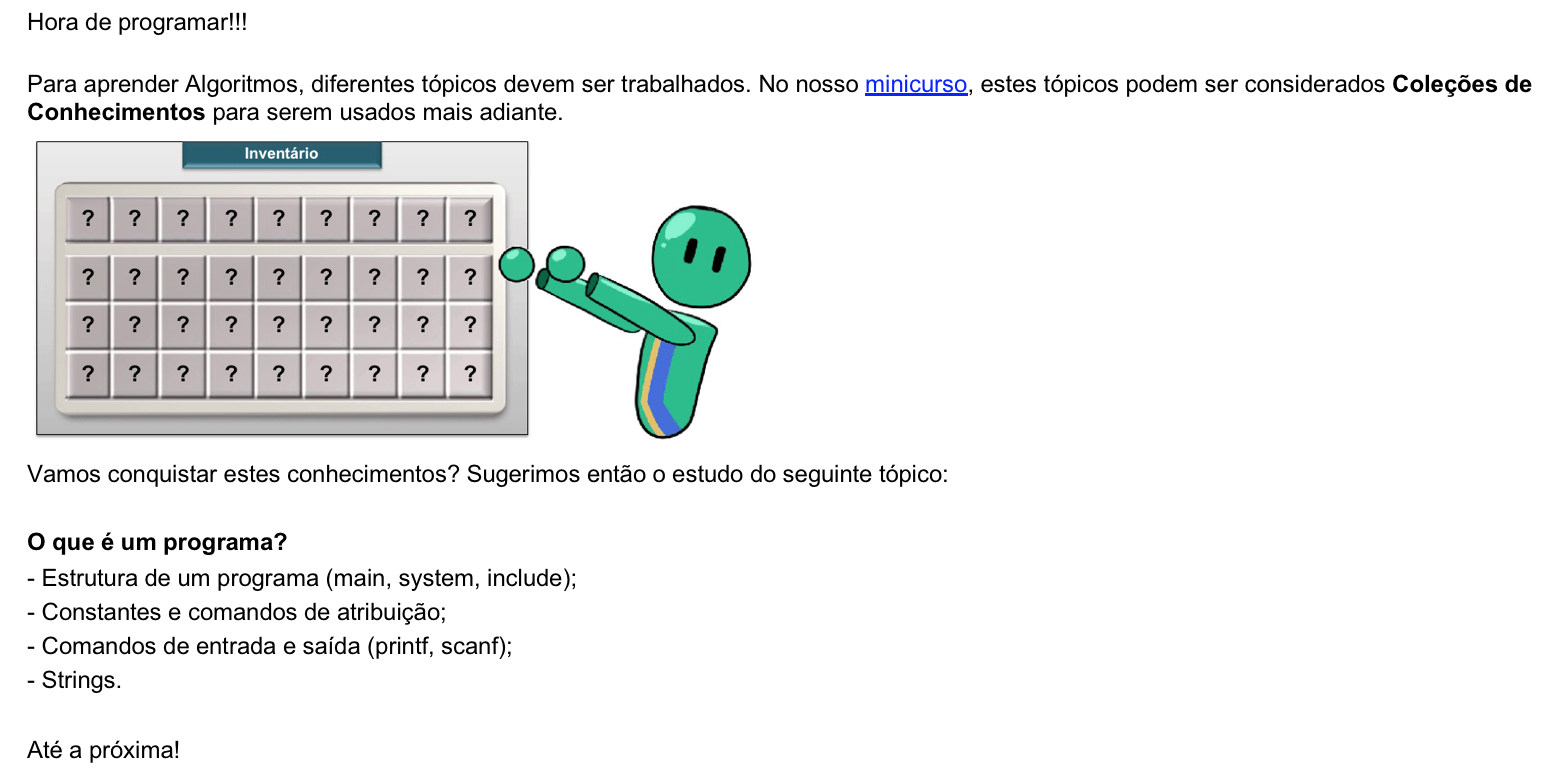
\includegraphics[scale=0.6]{./Figuras/intervencao-3.png}
  \end{center}
  \legend{Fonte: O autor.}
\end{figure}

\begin{figure}[htb]
  \caption{\label{fig:intervencao-4}Intervenção 4 (22/04/18)}
  \begin{center}
      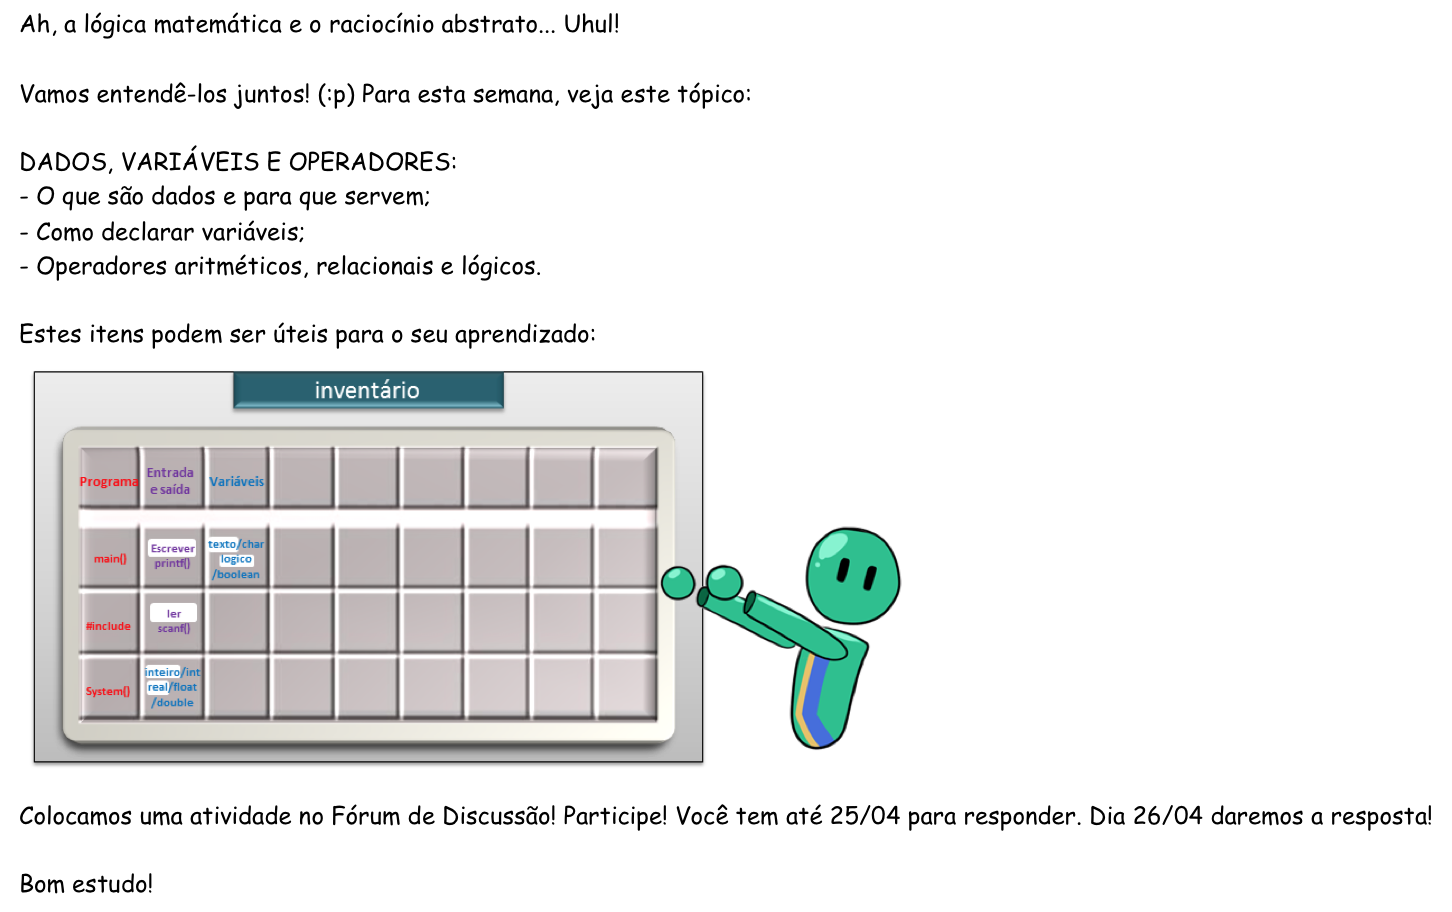
\includegraphics[scale=0.6]{./Figuras/intervencao-4.png}
  \end{center}
  \legend{Fonte: O autor.}
\end{figure}

\begin{figure}[htb]
  \caption{\label{fig:intervencao-5}Intervenção 5 (25/04/18)}
  \begin{center}
      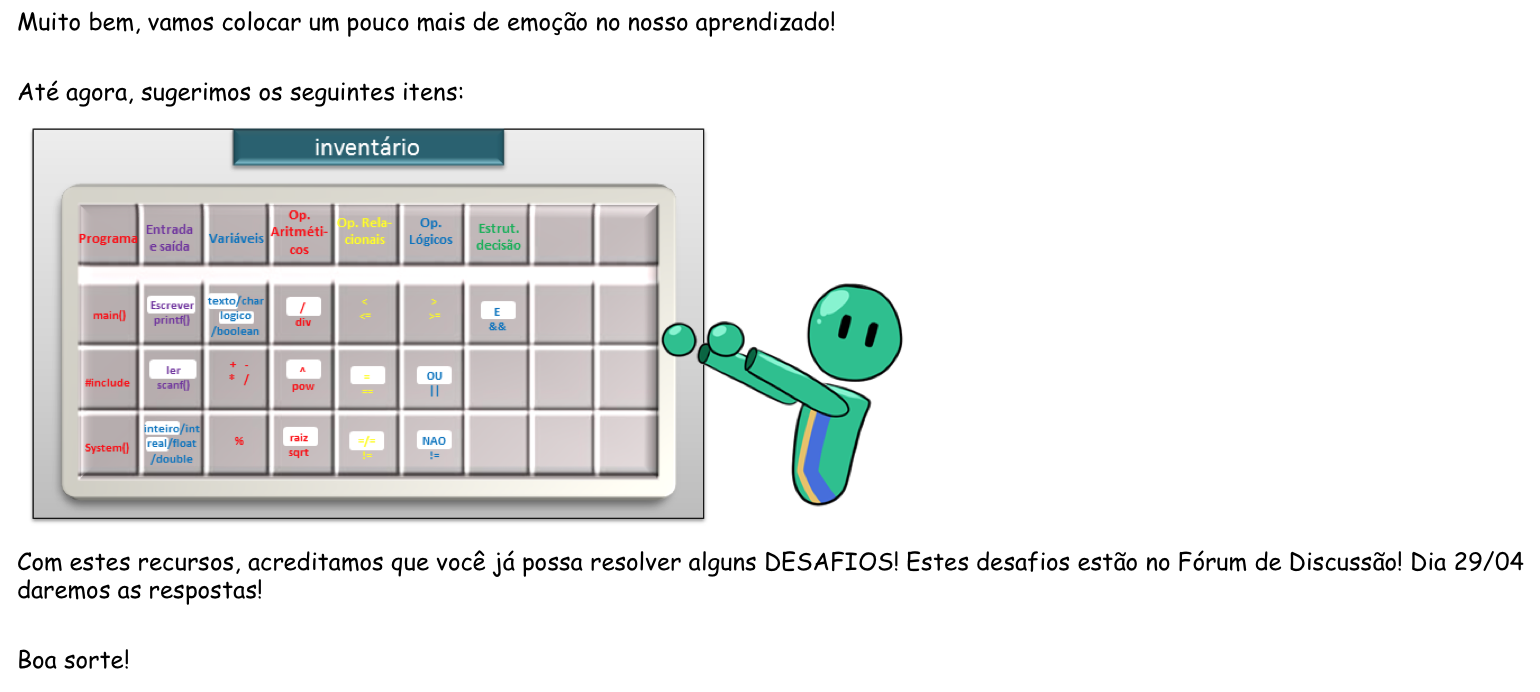
\includegraphics[scale=0.6]{./Figuras/intervencao-5.png}
  \end{center}
  \legend{Fonte: O autor.}
\end{figure}

\begin{figure}[htb]
  \caption{\label{fig:intervencao-6}Intervenção 6 (29/04/18)}
  \begin{center}
      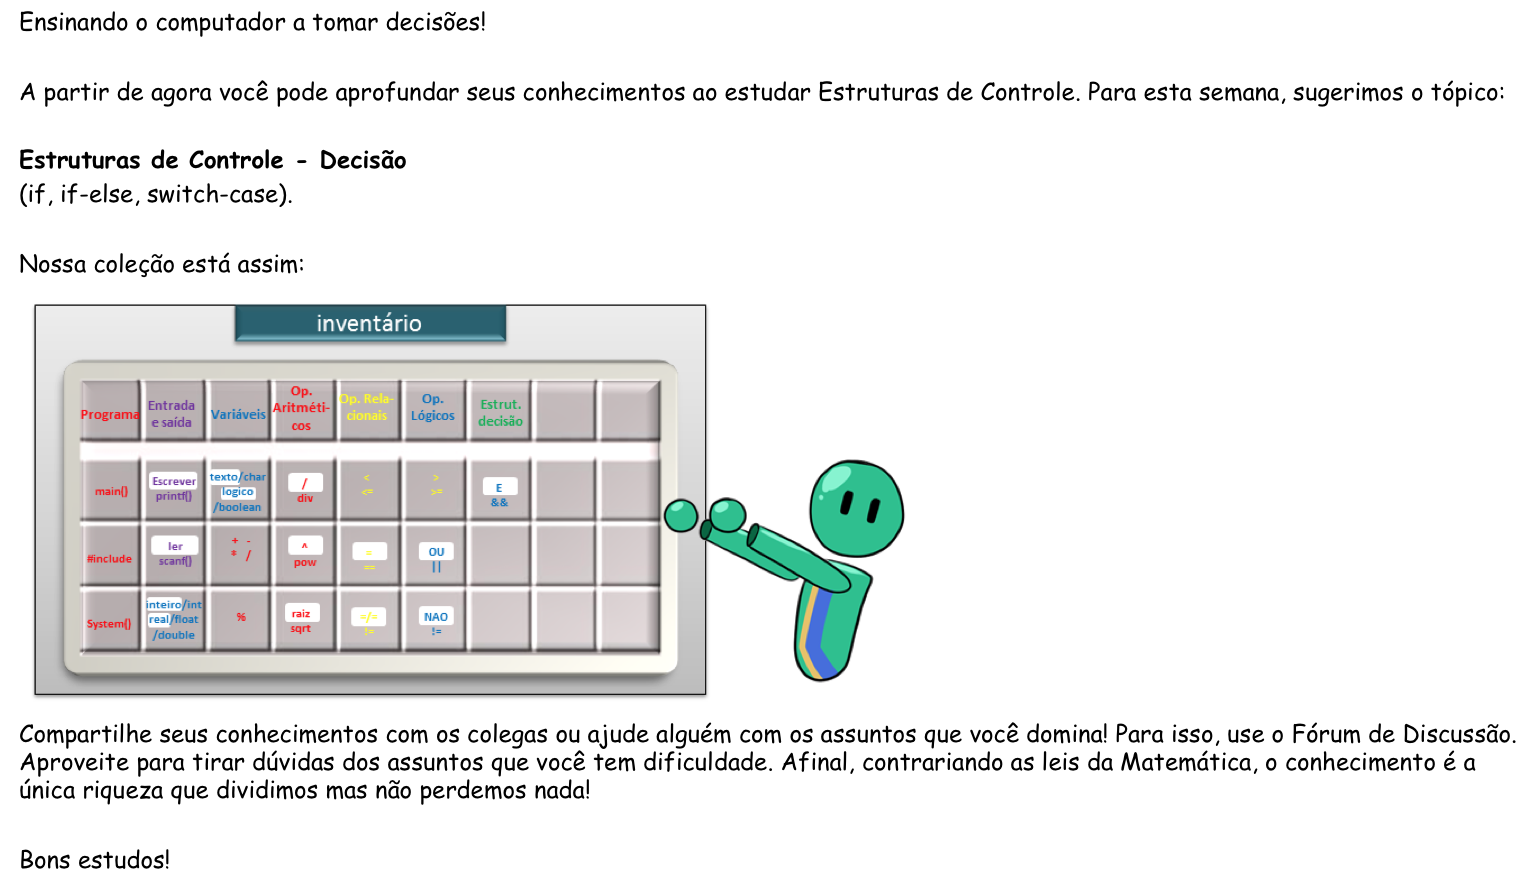
\includegraphics[scale=0.6]{./Figuras/intervencao-6.png}
  \end{center}
  \legend{Fonte: O autor.}
\end{figure}

\begin{figure}[htb]
  \caption{\label{fig:intervencao-7}Intervenção 7 (02/05/18)}
  \begin{center}
      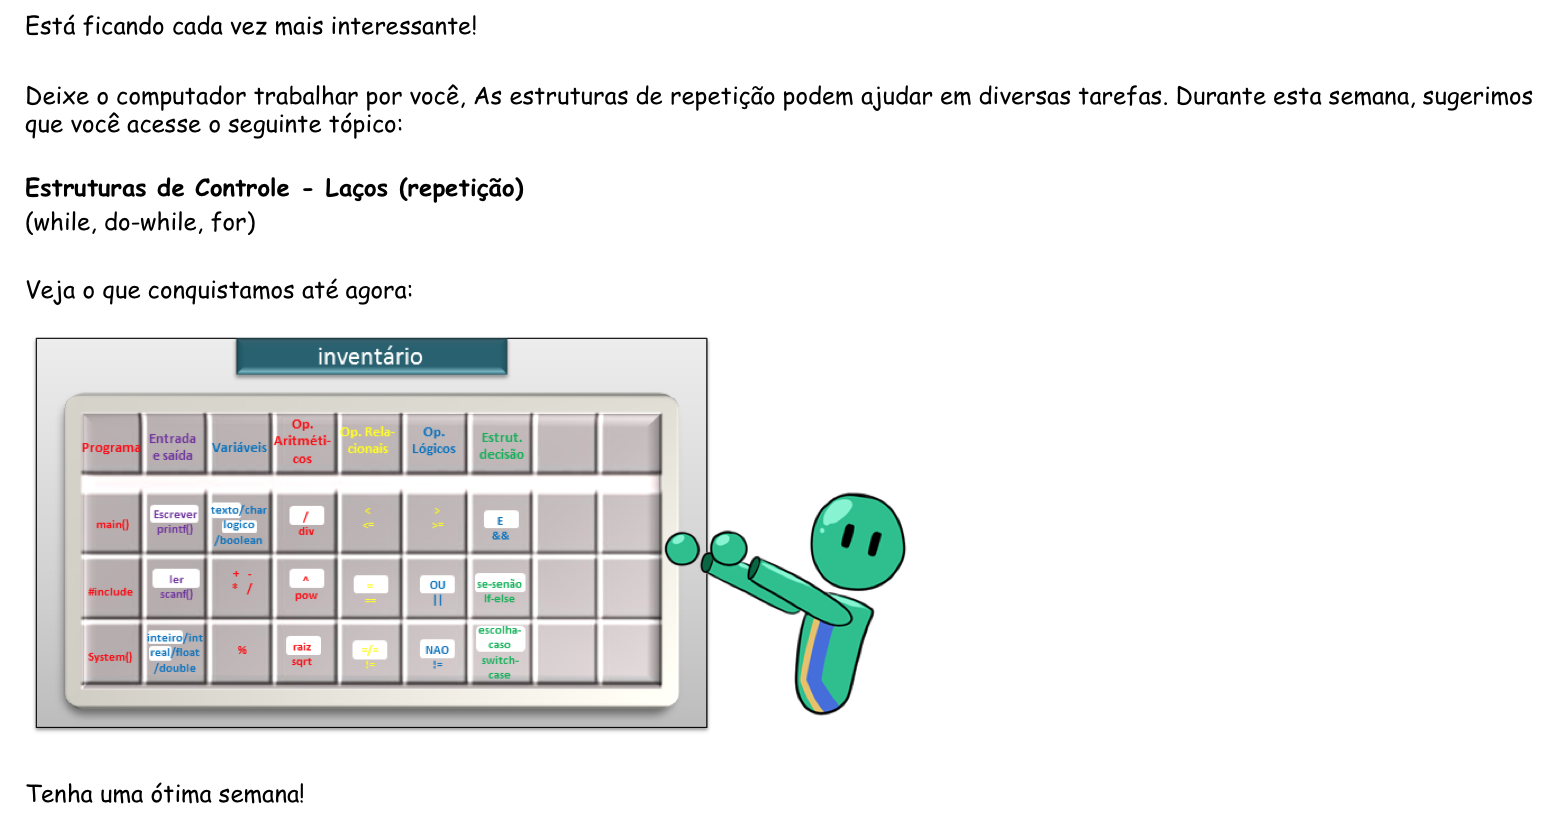
\includegraphics[scale=0.6]{./Figuras/intervencao-7.png}
  \end{center}
  \legend{Fonte: O autor.}
\end{figure}

\begin{figure}[htb]
  \caption{\label{fig:intervencao-8}Intervenção 8 (06/05/18)}
  \begin{center}
      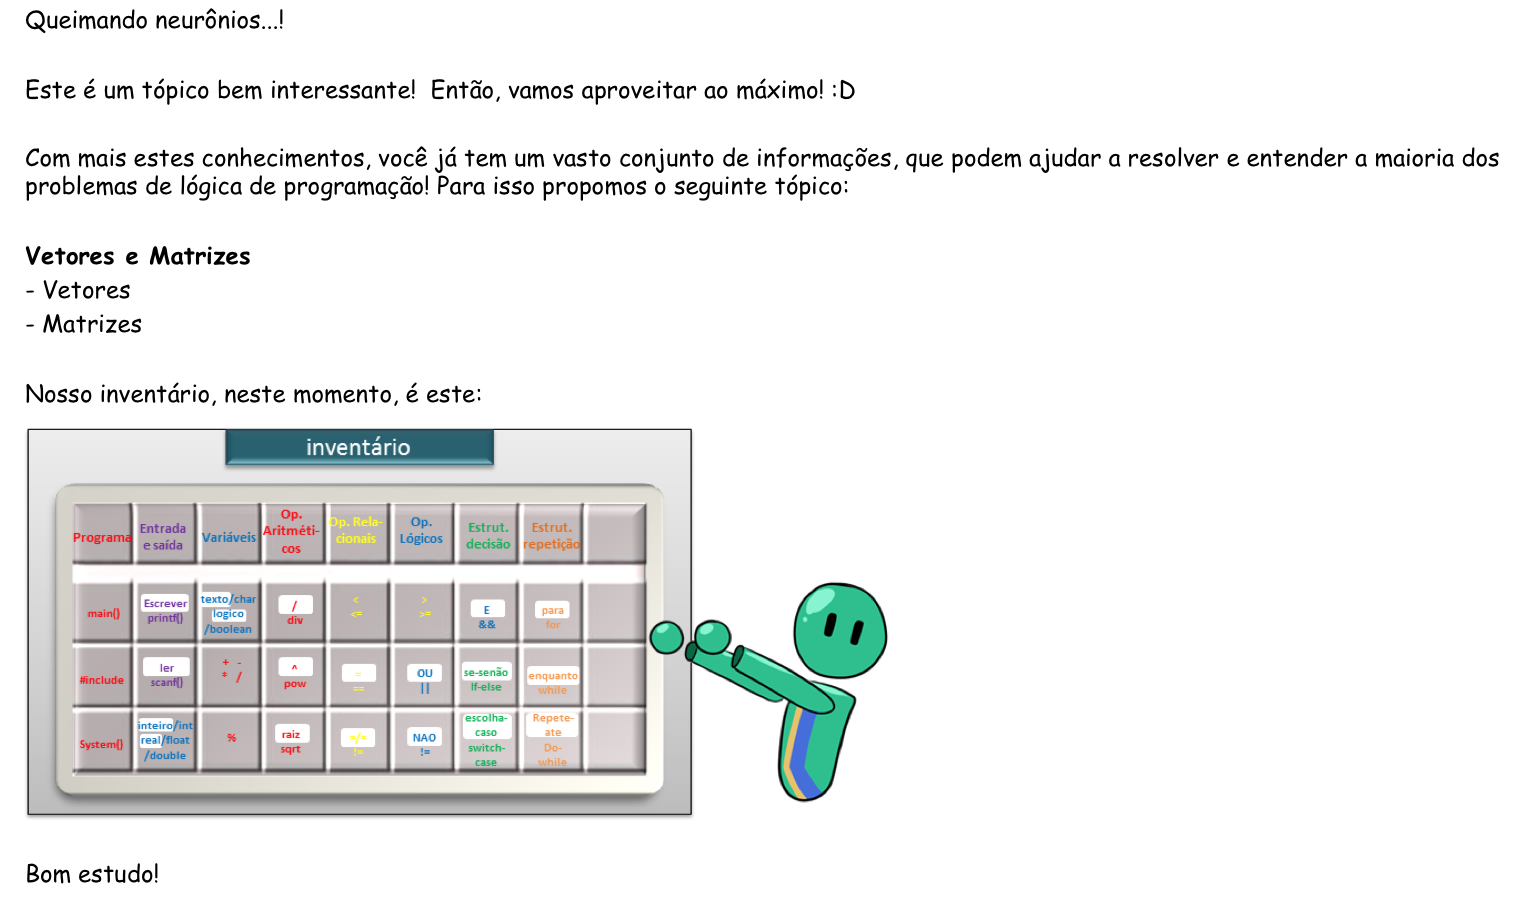
\includegraphics[scale=0.6]{./Figuras/intervencao-8.png}
  \end{center}
  \legend{Fonte: O autor.}
\end{figure}

\begin{figure}[htb]
  \caption{\label{fig:intervencao-9}Intervenção 9 (09/05/18)}
  \begin{center}
      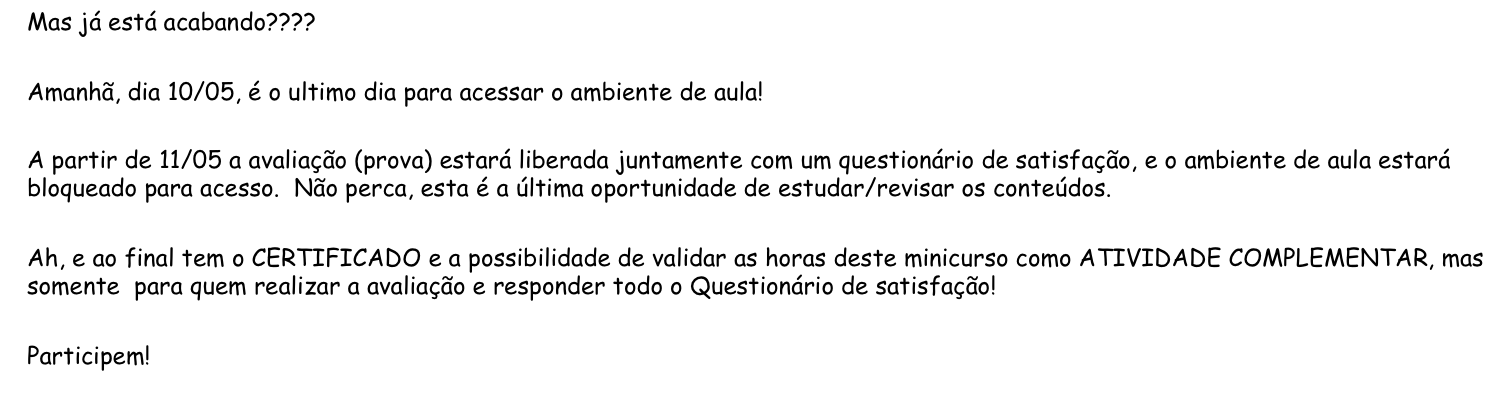
\includegraphics[scale=0.6]{./Figuras/intervencao-9.png}
  \end{center}
  \legend{Fonte: O autor.}
\end{figure}

\begin{figure}[htb]
  \caption{\label{fig:intervencao-10}Intervenção 10 (10/05/18)}
  \begin{center}
      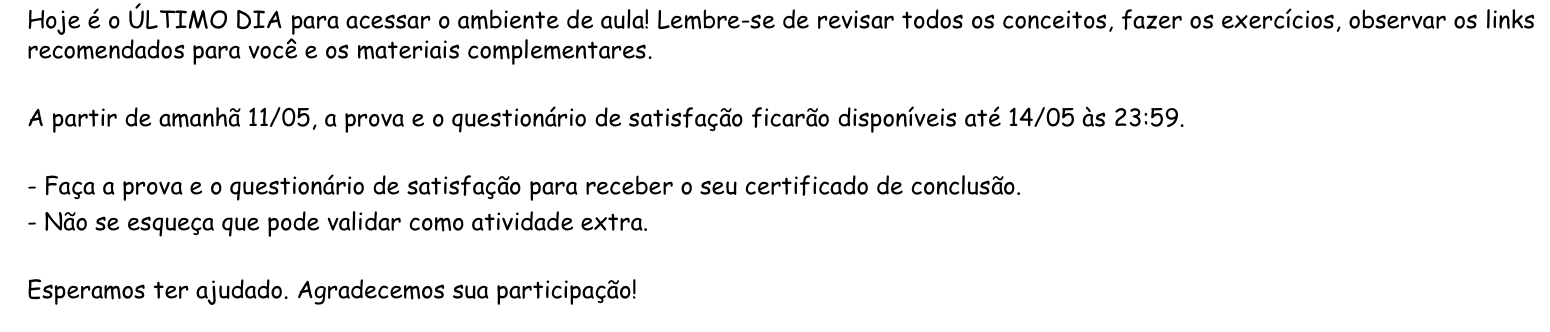
\includegraphics[scale=0.6]{./Figuras/intervencao-10.png}
  \end{center}
  \legend{Fonte: O autor.}
\end{figure}

\begin{figure}[htb]
  \caption{\label{fig:intervencao-11}Intervenção 11 (11/05/18)}
  \begin{center}
      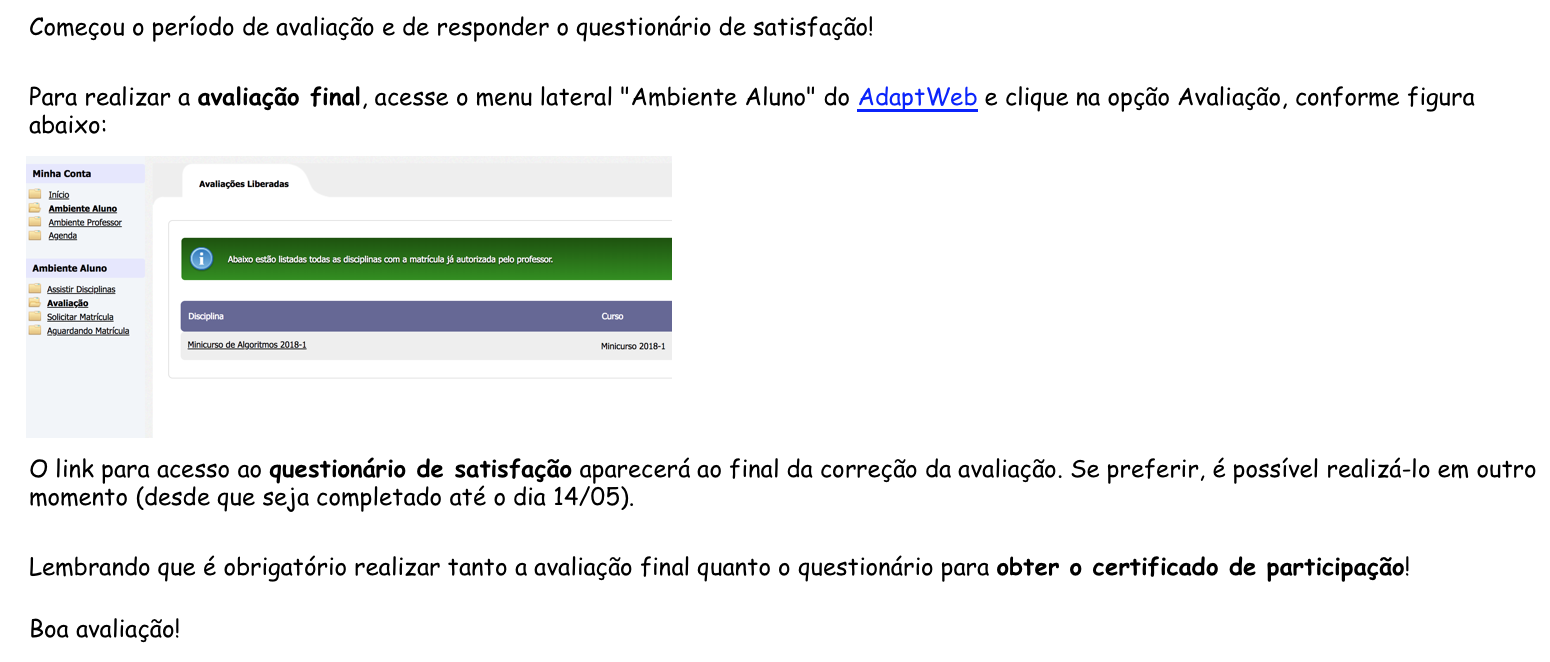
\includegraphics[scale=0.6]{./Figuras/intervencao-11.png}
  \end{center}
  \legend{Fonte: O autor.}
\end{figure}

\begin{figure}[htb]
  \caption{\label{fig:intervencao-12}Intervenção 12 (13/05/18)}
  \begin{center}
      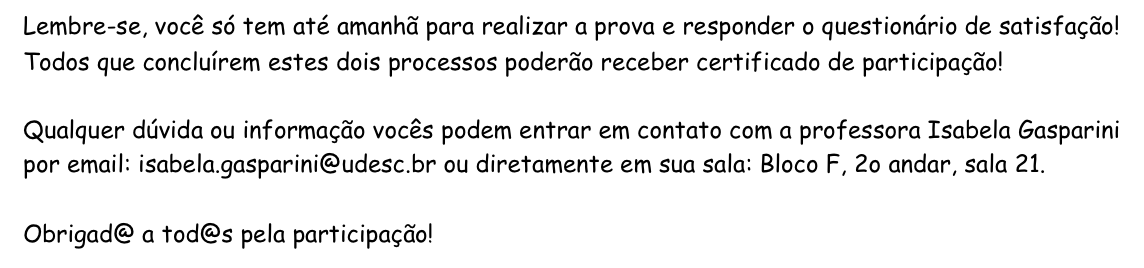
\includegraphics[scale=0.6]{./Figuras/intervencao-12.png}
  \end{center}
  \legend{Fonte: O autor.}
\end{figure}
